In this chapter we will deal with soliton solutions of systems of Calogero-Moser type introduced previously. We will define what exactly a soliton solution to an $N$-body problem is, and derive these solutions in a unified way for the systems presented in Chapter~\ref{ch:cm}, following \cite{philip2019soliton}. Lastly, we will study soliton solutions for the rational case with external harmonic potential (eCM), as done in \cite{kulkarni2017, abanov2011}, for different values of $N$. 

\section{Soliton solutions to many-body systems}
Let us first explain what we mean by a \textit{soliton solution}. 

\subsection{Soliton waves}
The word ``soliton'' was first introduced by N. J. Zabusky and M. D. Kruskal in \cite{zabusky1965}, in 1965. We call \textit{soliton} (or solitary wave) a phenomenon of localized non-linear waves bearing permanent form and propagating at constant speed. More formally,

\begin{defi}
A \textit{solitary wave solution} or \textit{soliton} is a solution to any wave equation that satisfies the following three properties:

\begin{enumerate}
    \item retains its shape for all time;
    \item is localized (asymptotically constant at $\pm \infty$);
    \item can pass through other solitons and retain size and shape.
\end{enumerate}
\end{defi}

The first soliton wave was observed by J. Scott Russell on the Edinburgh-Glasgow canal in 1834. His observations were reported in 1844 to the British Association in his ``Report on Waves'' \cite{russell1844}. In 1895 D. Korteweg and G. de Vries proposed a mathematical model for solitary waves, described by the KdV equation \cite{korteweg1895}, with wave profile $u(x,t)$:

\begin{equation}
    u_t - 6uu_x + u_{xxx} = 0\;,
\end{equation}

whose hyperbolic 1-soliton solution is

\begin{equation}\label{soliton}
    u(x,t) = a\sech^2{b (x - ct - x_0)}\;,
\end{equation}

where $c > 0$ is the speed, $a = -c/2$ and $b = \sqrt{c}/2$.

\subsection{Poles of nonlinear waves as interacting particles}
Soliton theory is closely related to the theory of integrable systems, because solitons are exact solutions to some equations of motion. We can show this connection by determining the poles $p_n(t)$ of (\ref{soliton}), as done in \cite{deconinckpole}:

\begin{equation}
p_n(t) = x_0 + ct + \frac{i\pi}{b} \Big (n + \frac{1}{2} \Big )\;,\;\;\;\;\;\;\;\;n \in \mathbb{Z}.
\end{equation}

The dynamics of the solitary wave is determined by the evolution of these poles. Interestingly, the motion of the poles corresponds formally to the motion of 1-dimensional particles interacting via simple two-body potentials (\cite{assis2009}). \\
Consider the Benjamin-Ono equation \cite{benjamin1967, ono1975}

\begin{equation}\label{benjaminono}
    u_t + \hat H u_{xx} + 2uu_x = 0\;,
\end{equation}

where $\hat H$ is the Hilbert transform

\begin{equation}
    \hat H[f](x) = \frac{\textnormal{p.v.}}{\pi}\int_{- \infty}^{+ \infty} \frac{f(z)}{x - z}dz\;,
\end{equation}

with $\textnormal{p.v.}$ the Cauchy principal value.  This model describes internal waves of permanent form in a deep fluid (see Figure~\ref{fig:gibraltar}). Such wave motion in the bulk of a fluid occurs because of density stratification \cite{bona2019}. In an idealized situation, where a homogeneous layer of light incompressible fluid rests upon a similar layer of heavier fluid, and surface tension and diffusion between the two layers as well as damping are ignored, the full equations for internal wave motion are usually taken to be a pair of inviscid, homogeneous fluids coupled through the interface. If the latter is far from the bounding surfaces, the rigid lid approximation can be legitimate in certain cases. 

\begin{figure}
    \centering
    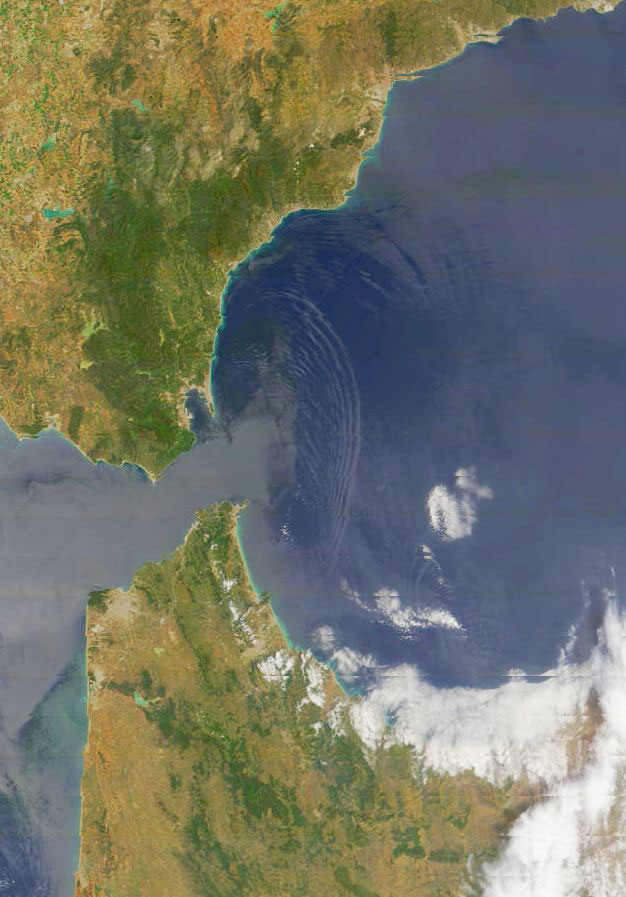
\includegraphics[width = 4cm]{images/internalwavesgibraltar.jpg}
    \caption{Internal waves in the Eastern Strait of Gibraltar. Source: \cite{eumetsat_2017}}
    \label{fig:gibraltar}
\end{figure}

A solution of (\ref{benjaminono}) has the form \cite{chen1979}

\begin{equation}
    u(x,t) = i\sum_{n=1}^N \Big ( \frac{1}{x - z_n(t)} - \frac{1}{x - z_n^\ast (t)} \Big )\;,
\end{equation}

whose poles satisfy the complex Calogero-Moser equations of motion

\begin{equation}
    \ddot z_n(t) = 8 \sum_{m=1,\;m \neq n}^N \frac{1}{(z_n(t) - z_m(t))^3}\;.
\end{equation}

More generally, the following holds \cite{philip2019soliton}.

\begin{thm}
Let $\alpha(x)$ be a special Lax function. The meromorphic functions 

\begin{equation}\label{solitonequation}
    u(x,t) = \sum_{j=1}^N \alpha (x - x_j) - \sum_{n=1}^M \alpha (x - z_n) - i\omega x\;,
\end{equation}

for arbitrary $N$ and $M$ form a class of solutions to equations of Benjamin-Ono type (the equation (\ref{benjaminono}) itself in the rational case with $\omega = 0$, see \cite{philip2019soliton} for the other cases) if and only if their poles $\{x_j\}$ and $\{z_n\}$ satisfy the system of equations

\begin{subequations}
\begin{align}[left=\empheqlbrace]
\dot x_j &= - \sum_{k=1,\;k \neq j}^N \alpha(x_j - x_k) + \sum_{n = 1}^M \alpha(x_j - z_n) + \lambda + i\omega x_j\;,\\
\dot z_n &= \sum_{m=1,\;m \neq n}^M \alpha(z_n - z_m) - \sum_{l = 1}^N \alpha(z_n - x_l) + \lambda + i\omega z_n\;,
\end{align}
\end{subequations}

where $\lambda$ and $\omega$ are constants. 
\end{thm}

We can operate a finite-dimensional reduction of such infinite-dimensional systems. Given a solution of that system of the form $u(x,t)$ we can consider a discretization $u(x; \{z_n\})$ so that the time dependence of $u$ is reduced to $M$ complex parameters $z_n (t)$, with $n = 1, 2,..., M$ with known time dependence. We call $u(x, \{z_n(t)\})$ for $n = 1, ..., M$ an $M$-soliton solution \cite{abanov2011}. 

\section{General method}\label{sec:general}
Consider $N$ complex canonical coordinates $x_j = q_j, \dot x_j = p_j \in \mathbb{C}$ and $M$ canonical coordinates $z_n, \dot z_n \in \mathbb{C}$ and their respective Hamiltonians

\begin{subequations}
\begin{align}
    \mathcal{H} &= \frac{1}{2}\sum_j ({\dot x_j}^2 + \omega^2 x_j^2) + \sum_{j < k} V(x_j - x_k), \\
    \mathcal{H'} &= \frac{1}{2}\sum_n ({\dot z_n}^2 + \omega^2 z_n^2) + \sum_{n < m} V(z_n - z_m)\;,
\end{align}
\end{subequations}

with 

\[V(x) = \left \{ \begin{array}{cc}
{g^2}/{x^2}  & \textnormal{(I)}\\
{g^2a^2}/{\sin^2{ax}}  & \textnormal{(II)}\\
{g^2a^2}/{\sinh^2{ax}} & \textnormal{(III)}
\end{array}
\right.\]

In the literature, $\{x_j\}$ is often called the \textit{principal system} and $\{z_n\}$ the \textit{auxiliary system} or the \textit{dual Calogero-Moser system}. From now on we write the special Lax function as $i\alpha(x)$, with $\alpha(x) = g/x$, $ga/\sin{ax}$ or $ga/\sinh{ax}$, which is real on the real axis. Then a subset of the solutions to each system can be connected by a Bäcklund transformation of the form

\begin{subequations}
\begin{align}[left=\empheqlbrace]
\dot x_j &= - i\sum_{k=1,\;k \neq j}^N \alpha(x_j - x_k) + i\sum_{n = 1}^M \alpha(x_j - z_n) + i\omega x_j \label{soliton1}\;,\\
\dot z_n &= i\sum_{m=1,\;m \neq n}^M \alpha(z_n - z_m) - i\sum_{l = 1}^N \alpha(z_n - x_l) + i\omega z_n\label{soliton1b}\;.
\end{align}
\end{subequations}

\begin{obs}
Taking the time derivative of (\ref{soliton1}) and (\ref{soliton1b}) and using (\ref{soliton1}) and (\ref{soliton1b}) again, we obtain the decoupled systems of second-order ODEs

\begin{subequations}
\begin{align}
    \ddot x_j &= - \frac{\partial }{\partial x_j} \sum_{i = 1,\; i \neq j}^N V(x_i - x_j) - \omega^2 x_j \\
    \ddot z_n &= - \frac{\partial }{\partial z_n} \sum_{m = 1,\; m \neq n}^M V(z_m - z_n) - \omega^2 z_n\;,
\end{align}
\end{subequations}

that are the equations of motion of the two systems considered. 
\end{obs}

For $M < N$, the principal system is reduced via the Bäcklund transformation into a system with fewer degrees of freedom. \\
If $x_j, p_j = \dot x_j \in \mathbb{R} \;\forall j$ (real reduction), (\ref{soliton1}) may be split into two equations concerning separately real and imaginary parts:

\begin{subequations}
\begin{align}[left=\empheqlbrace]
    \sum_{k=1,\;k \neq j}^N \alpha (x_j - x_k) &= \sum_{n=1}^M \operatorname{Re}{\alpha(x_j - z_n)} + \omega x_j \label{soliton2}\;, \\
    \dot x_j &= - \sum_{n = 1}^M \operatorname{Im}{\alpha(x_j - z_n)} \label{soliton3}\;.
\end{align}
\end{subequations}

For $M$ given initial conditions $\{z_n(0)\}$, one can find both $N$ real positions $\{x_j(0)\}$ solving numerically (\ref{soliton2}), and the corresponding real momenta $\{\dot x_j(0)\}$ using (\ref{soliton3}) \cite{philip2019soliton}. Then, the evolutions of the soliton solutions are completely and independently determined by the Olshanetsky-Perelomov projection method, due to the eigenvalues' invariance.

\section{1-soliton solutions for eCM}
Let us apply the general method to the special case of the rational potential with external harmonic potential (eCM). For $M = 1$ the Bäcklund transformations read

\begin{subequations}
\begin{align}[left=\empheqlbrace]
\dot x_j &= -ig \sum_{k=1,\;k \neq j}^N \frac{1}{(x_j - x_k)} + ig \frac{1}{(x_j - z)} + i\omega x_j \label{soliton4}\;,\\
\dot z &= - ig \sum_{l=1}^N \frac{1}{(z - x_l)} + i\omega z\;.
\end{align}
\end{subequations}

Separating (\ref{soliton4}) into its real and imaginary parts, we get

\begin{subequations}
\begin{align}[left=\empheqlbrace]
    \omega x_j &= g\sum_{k=1,\;k \neq j}^N \frac{1}{x_j - x_k} - g \operatorname{Re}{\frac{1}{x_j - z}} \label{soliton5}\;, \\
    \dot x_j &= - g \operatorname{Im}{\frac{1}{x_j - z}} \label{soliton6}\;.
\end{align}
\end{subequations}

Solving numerically (\ref{soliton5}) for a given initial condition $z(0)$, we find $N$ real positions $\{x_j(0)\}$, and then the corresponding real momenta $\{\dot x_j(0)\}$ using (\ref{soliton6}). The evolutions of the soliton solutions are determined by the Olshanetsky-Perelomov procedure: $\{x_j(t)\}$ and $\{z(t)\}$ are given respectively by the eigenvalues of the matrix

\begin{equation}
    X_{jk} (t) = \delta_{jk} \Big (\dot x_j(0)\frac{\sin{\omega t}}{\omega} + x_j (0)\cos{\omega t} \Big ) + (1 - \delta_{jk}) ig \frac{\sin{\omega t}}{\omega(x_j(0) - x_k(0))}\;,
\end{equation}

and by the equation of motion

\begin{equation}
    z(t) = \Big (\dot z(0)\frac{\sin{\omega t}}{\omega} + z(0)\cos{\omega t} \Big ) \;.
\end{equation}

Solving the system numerically\footnote{We use the function \texttt{FindRoot} in Wolfram Mathematica 13.}, we get the worldlines for the real system.

\begin{figure}[H]
    \centering
    \worldlines{data/fig3_2.csv}{10}{12cm}{7.5cm}
    \caption{Worldlines of the real $\textnormal{I}^+$ system for $N = 10$ particles, with $\omega = g = 1$ and initial value $z(0) = 1 + i$.}
    \label{fig:my_label}
\end{figure}

The soliton wave propagates along the real axis in coordination with the complex orbit $z(t)$. The soliton wave appears to propagate with constant speed (the shifts appear to be regularly spaced in time). The soliton excitation corresponds to the upward or downward shifts in the worldlines.  

\begin{figure}[H]
\centering
\begin{subfigure}{.49\textwidth}
  \centering
  \worldlines{data/fig3_3a.csv}{10}{\linewidth}{0.75\linewidth}
  \caption{}
  \label{fig:sub1}
\end{subfigure}%
\begin{subfigure}{.49\textwidth}
  \centering
  \worldlines{data/fig3_3b.csv}{10}{\linewidth}{0.75\linewidth}
  \caption{}
  \label{fig:sub2}
\end{subfigure}
\caption{Worldlines of the real $\textnormal{I}^+$ system for $N = 10$ particles, with $\omega = g = 1$ and initial values $z(0) = 1.2 + 0.3i$ for \ref{fig:sub1} and $z(0) = 2.8 + 2.4i$ for \ref{fig:sub2}.}
\label{fig:test}
\end{figure}

In Figure~\ref{fig:test} we can observe that if $z(0)$ is closer to the real axis, it yields a tighter orbit and more pronounced wave, while $z(0)$ farther gives the opposite behaviour, as confirmed by \cite{philip2019soliton}.

\section{$M$-soliton solutions for eCM}
We can apply the general method to the rational potential with external harmonic potential (eCM) for a generic $M < N$:

\begin{subequations}
\begin{align}[left=\empheqlbrace]
\dot x_j &= -ig \sum_{k=1,\;k \neq j}^N \frac{1}{(x_j - x_k)} + ig \sum_{n = 1}^M \frac{1}{(x_j - z_n)} + i\omega x_j \label{soliton7}\;,\\
\dot z_n &= ig \sum_{m=1,\;m\neq n}^M \frac{1}{z_n - z_m} - ig \sum_{l=1}^N \frac{1}{(z_n - x_l)} + i\omega z_n\;.
\end{align}
\end{subequations}

Separating (\ref{soliton7}) into its real and imaginary parts, we get

\begin{subequations}
\begin{align}[left=\empheqlbrace]
    \omega x_j &= g\sum_{k=1,\;k \neq j}^N \frac{1}{x_j - x_k} - g \sum_{n=1}^M\operatorname{Re}{\frac{1}{x_j - z_n}} \label{soliton8}\;, \\
    \dot x_j &= - g \sum_{n=1}^M\operatorname{Im}{\frac{1}{x_j - z_n}} \label{soliton9}\;.
\end{align}
\end{subequations}

Solving numerically (\ref{soliton8}) for $M$ given initial conditions $\{z_n(0)\}$, we find $N$ real positions $\{x_j(0)\}$, and then the corresponding real momenta $\{\dot x_j(0)\}$ using (\ref{soliton9}). The evolutions of the soliton solutions $\{x_j(t)\}$ and $\{z_n(t)\}$ are given by the eigenvalues of the matrices

\begin{subequations}
\begin{align}
    X_{jk} (t) &= \delta_{jk} \Big (\dot x_j(0)\frac{\sin{\omega t}}{\omega} + x_j (0)\cos{\omega t} \Big ) \nonumber\\ &\quad + (1 - \delta_{jk}) ig \frac{\sin{\omega t}}{\omega(x_j(0) - x_k(0))}\;, \\
    Z_{nm} (t) &= \delta_{nm} \Big (\dot z_n(0)\frac{\sin{\omega t}}{\omega} + z_n (0)\cos{\omega t} \Big ) \nonumber\\ &\quad + (1 - \delta_{nm}) ig \frac{\sin{\omega t}}{\omega(z_n(0) - z_m(0))}\;.
\end{align}
\end{subequations}

We present the results obtained numerically for $M = 2$. 

\begin{figure}[H]
\centering
\begin{subfigure}{.49\textwidth}
  \centering
  \worldlines{data/fig3_4a.csv}{6}{\linewidth}{0.75\linewidth}
  \caption{}
  \label{2soliton61}
\end{subfigure}%
\begin{subfigure}{.49\textwidth}
  \centering
  \worldlines{data/fig3_4b.csv}{6}{\linewidth}{0.75\linewidth}
  \caption{}
  \label{2soliton62}
\end{subfigure}
\caption{Worldlines of the real $\textnormal{I}^+$ system for $N = 6$ particles, with $\omega = g = 1$ and initial values $z_1(0) = -1.1 + 0.5i, z_2(0) = 0.1 -2i$ for \ref{2soliton61} and $z_1(0) = -1.1 + 0.5i, z_2(0) = 0.1 - i$ for \ref{2soliton62}.}
\end{figure}

For $M > 1$, we can note the effects of interaction between multiple solitons. The trajectories are deformed more or less significantly depending on the degrees of freedom of the dual system and the initial conditions.  

\begin{figure}[H]
\centering
\begin{subfigure}{.49\textwidth}
  \centering
  \worldlines{data/fig3_5a.csv}{6}{\linewidth}{0.75\linewidth}
  \caption{}
  \label{2soliton63}
\end{subfigure}%
\begin{subfigure}{.49\textwidth}
  \centering
  \worldlines{data/fig3_5b.csv}{6}{\linewidth}{0.75\linewidth}
  \caption{}
  \label{2soliton64}
\end{subfigure}
\caption{Worldlines of the real $\textnormal{I}^+$ system for $N = 6$ particles, with $\omega = g = 1$ and initial values $z_1(0) = 0.1 + 0.5i, z_2(0) = 0.1 -0.9i$ for \ref{2soliton63} and $z_1(0) = 0.1 + 0.5i, z_2(0) = 0.1 - 0.1i$ for \ref{2soliton64}.}
\end{figure}

\begin{figure}[H]
    \centering
    \worldlines{data/fig3_6.csv}{10}{12cm}{7.5cm}
    \caption{Worldlines of the real $\textnormal{I}^+$ system for $N = 10$ particles, with $\omega = g = 1$ and initial values $z_1(0) = 0.1 + 0.5i, z_2(0) = 0.1 - i$.}
    \label{figsoliton10}
\end{figure}

\begin{obs}
As noted by \cite{abanov2011} and reported in \cite{kulkarni2017, philip2019soliton}, soliton solutions to the rational CM system correspond to extremal conditions of an electrostatic energy function $E$. In fact, considering the Coulomb potential $V(x_j - z_n) = \ln{|x_j - z_n|} = \frac{1}{2}\big[\ln{(x_j - z_n)} + \ln{(x_j - \bar z_n)}\big]$, we get

\begin{equation}
    \frac{\partial V(x_j - z_n)}{\partial x_j} = \frac{1}{2} \Big ( \frac{1}{x_j - z_n} + \frac{1}{x_j - \bar z_n} \Big ) = \operatorname{Re}{\frac{1}{x_j - z_n}}\;.
\end{equation}

Then, given $E$ the potential of the system

\begin{equation}
    E = \sum_{j=1}^N \frac{\omega x_j^2}{2} - g \sum_{1 \leq j < k \leq N} \ln{|x_j - x_k|} + \frac{g}{2} \sum_{j = 1}^N \sum_{n=1}^M \ln{|x_j - z_n|^2}\;,
\end{equation}

it follows

\begin{equation}
    \frac{\partial E}{\partial x_j} = \omega x_j - g \sum_{k=1,\;k \neq j}^N \frac{1}{x_j - x_k} + g\sum_{n=1}^M \operatorname{Re}{\frac{1}{x_j - z_n}}\;.
\end{equation}

Hence, equation (\ref{soliton8}) can be derived from the extremal condition 

\begin{equation}
    \frac{\partial E}{\partial x_j} = 0\;.
\end{equation}

In this view, the positive charges $\{z_n\}$ interact with the negative charges $\{x_j\}$ on the line, inducing the soliton wave. 
\end{obs}

\section{Conclusions}
In Section~\ref{sec:general} we described, following \cite{philip2019soliton}, a general method to find soliton solutions to a variety of systems of Calogero-Moser type (in particular, systems of class I, II, III and $\textnormal{I}^+$). The method takes advantage of the unified description of these systems in terms of their Bäcklund transformations, which depend on a single special Lax function $\alpha(x)$, as seen in Chapter~\ref{ch:cm}. We saw that Bäcklund transformations and $M$-soliton solutions reduce the number of degrees of freedom of the systems considered: it is sufficient to specify $M$ initial conditions for the dual $M$-dimensional system $\{z_n\}$ to determine the dynamics of the real CM system with $N$ degrees of freedom, for the generic $N$. Finally, we presented some numerical examples of $M$-soliton solutions for $M = 1, 2$ for the rational CM system with external harmonic potential (eCM or $\textnormal{I}^+$).  